The \emph{PanicButton device} has to perform tasks like take user's input from the panic button, acquire audio data needed for audio-based trigger, communicate with the back-end server and user's smartphone, detect any tampering and run audio processing algorithms. Figure~\ref{fig:functionalDesc} and  figure~\ref{fig:functionalDescbus} shows the top level functional diagram of the \emph{PanicButton device} when installed in cabs/autos and bus respectively.

\emph{PanicButton device} is equipped with a panic button to take user inputs, bluetooth low energy (BLE) for communicating with the user's smartphone, global system for mobile communication (GSM) to communicate with back-end server, global positioning system (GPS) to locate the vehicle in case of emergency, microphone to record audio and speaker to play audio.

Users can validate \emph{PanicButton device} using their smartphone through a dedicated android application. Communication between the user's smartphone and the \emph{PanicButton device} is handled by the respective BLE module. After performing validation, user is notified with the status of microphone, emergency button, firmware and enclosure of the system.

%\begin{figure}[H]
%\centering
%\def\svgwidth{\textwidth}
%\input{functionalDescription.pdf_tex}
%\caption{Functional description of connected panic button with audio-based trigger}
%\label{fig:functionalDesc}
%\end{figure}

%\begin{figure}[H]
%\centering
%\def\svgwidth{\textwidth}
%\input{bus.pdf_tex}
%\caption{Functional description of connected panic button with audio-based trigger inside a bus}
%\label{fig:functionalDescbus}
%\end{figure}
\begin{figure}[H]
\centering
\def\svgwidth{\textwidth}
\includegraphics[width=0.9\textwidth]{functionalDescription}
\caption{Functional description of the \emph{PanicButton device} with audio-based trigger in auto/cab}
\label{fig:functionalDesc}
\end{figure}

\begin{figure}[H]
\centering
\def\svgwidth{\textwidth}
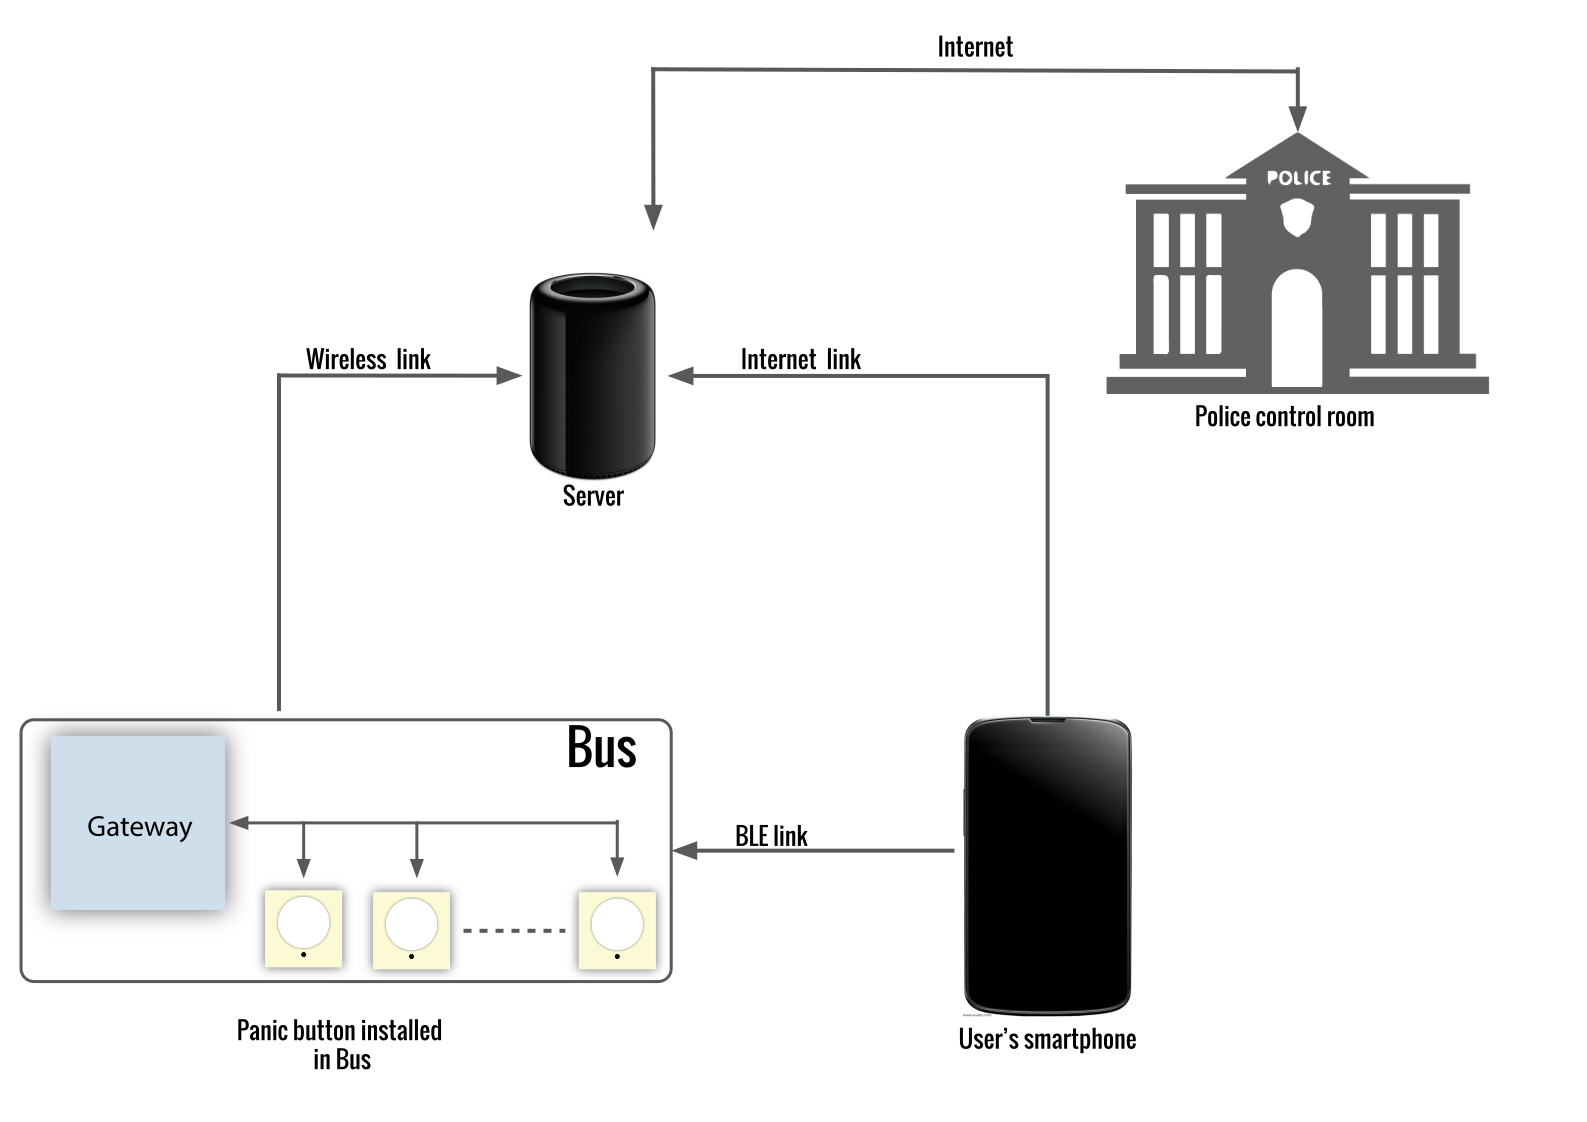
\includegraphics[width=0.9\textwidth]{bus}
\caption{Functional description of the \emph{PanicButton device} with audio-based trigger in bus}
  \label{fig:functionalDescbus}
\end{figure}

Emergency is asserted, if either the panic button is pressed or scream is detected by audio-based trigger. In case of emergency, compressed stream of audio along with vehicle's location is sent to the server, for later examination.

